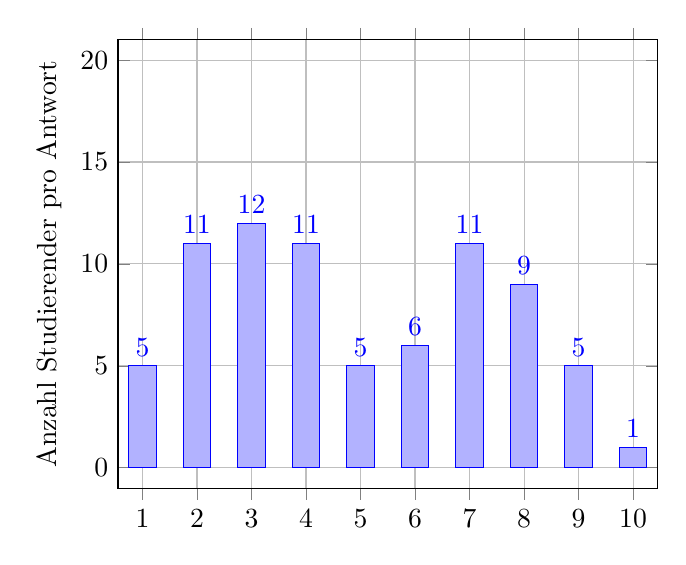
\begin{tikzpicture}
    \begin{axis}[
    	x tick label style={
    		/pgf/number format/1000 sep=},
    	ylabel=Anzahl Studierender pro Antwort,
    	enlargelimits=0.05,
        ymax=20,
        ymin=0,
    	ybar,
        xtick=data,
        xticklabels={1,2,3,4,5,6,7,8,9,10},
        grid=major,
        nodes near coords,
    ]
    \addplot 
    	coordinates {(1,5) (2,11)
    		  (3,12) (4,11) (5,5) (6,6) 
            (7,11) (8,9) (9,5) (10,1)};
    \end{axis}
\end{tikzpicture}